\documentclass[a4paper,norsk,12pt]{article}
\usepackage[utf8]{inputenc}

% Oppsett for norsk
\usepackage[norsk]{babel}
\usepackage{times}
\usepackage[T1]{fontenc}
\usepackage{parskip}
\DeclareUnicodeCharacter{00A0}{ }
\newcommand{\strek}{\textthreequartersemdash}

% Andre pakker
\usepackage{oving}
\usepackage{amsmath}
\usepackage{amssymb}
\usepackage{varioref}
\usepackage{subcaption}
\usepackage{units}
\usepackage{todo}

\def \oppgavename {Problem}

% Roman numerals
\makeatletter
\newcommand*{\rom}[1]{\expandafter\@slowromancap\romannumeral #1@}
\makeatother


\title{MAT200 --- Mathematical Methods 2}
\subtitle{Compulsory Assignment 1}
\author{Christian Stigen}
\date{UiS, 19.~februar, 2016}

\begin{document}
\maketitle

\oppgave{1 (i)}
\label{problem.1}

The radicand must be zero or greater, or
\begin{align*}
  0 & \leqslant x^2-6x+\frac{1}{4}y^2 \> \Big{|} \cdot-4 \\
  0 & \geqslant 4x(6-x)-y^2 \\
  y^2 & \geqslant 4x(6-x)
\end{align*}
The right-hand side is zero for $x=0$ and $x=6$, and negative for $x<0$
and $x>6$. Thus, the inequality is true for $0 < x < 6$.

For plotting $\mathcal{D}(f)$, we note that
  \begin{align}
    y_{-} \leqslant -2\sqrt{x(6-x)} & \wedge y_{+} \geqslant 2\sqrt{x(6-x)}
    \,\text{for}\, 0<x<6 \label{eq.1i}
  \end{align}
In fact, taken together, they form an ellipse (see figure \vref{plot.p1}).

\oppgave{1 (ii)}

$C=0$ is given by (\ref{eq.1i}) above,
\begin{align*}
  f(x,y) = \sqrt{x^2 - 6x + \frac{1}{4}y^2} &= 0\\
  x^2 - 6x + \frac{1}{4}y^2 &= 0\\
  y = \pm2\sqrt{x(6-x)} \, \text{for} \, &0 \leqslant x \leqslant 6
\end{align*}
$C=4$ is given by
\begin{align*}
  f(x,y) &= \sqrt{x^2 - 6x + \frac{1}{4}y^2} = 4\\
  \frac{1}{4}y^2 &= 16 - x^2 + 6x\\
  y &= \pm2\sqrt{(x+2)(8-x)}
\end{align*}

The plot of these two level-curves (or \textit{contour curves}) is given in figure
\vref{plot.p2}. Note that we could have used scaling and shifting, which is
much easier, but I felt like doing it this way for fun.

\oppgave{1 (iii)}
First we need to find an expression of the level curve $g$ passing through $(x_0,
y_0) = (5,6)$. Using the implicit derivative $g'$, the tangent line in $(x_0,
y_0)$ is described by
\begin{align*}
  T(x) &= y_0 - x_0 g'(x_0, y_0) + xg'(x_0, y_0) \\
       &= y_0 + g'(x_0, y_0)\left( x - x_0 \right)
\end{align*}

To find the level curve, we go through a constant $C$.
\begin{align*}
  C &= \sqrt{x_0^2 - 6x_0 + \frac{1}{4}y_0^2} \\
  C^2 &= x_0^2 - 6x_0 + \frac{1}{4}y_0^2 \\
  C^2 &= 4 \\
  C &= 2
\end{align*}
This gives us $g$,
\begin{align*}
  4 &= x^2 - 6x + \frac{1}{4}y^2 \\
  g(x,y) &= x^2 - 6x + \frac{1}{4}y^2 - 4 \\
\end{align*}

\begin{figure}[h]
  \centering
  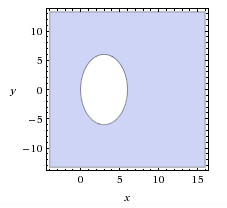
\includegraphics{ob1plot.png}
  \caption{Plot of $\mathcal{D}(f)$ in problem 1 (i).}
  \label{plot.p1}
\end{figure}

\begin{figure}[h]
  \centering
  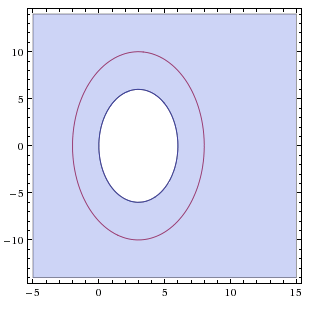
\includegraphics{ob1plot2.png}
  \caption{Plot of $f=0$ and $f=4$ in problem 1 (ii).}
  \label{plot.p2}
\end{figure}

\oppgave{2 (i)}

\oppgave{2 (ii)}

\oppgave{2 (iii)}

\oppgave{3 (i)}

\oppgave{3 (ii)}

\oppgave{3 (iii)}

\oppgave{3 (iv)}

\begin{align*}
  F(0,y) &= 1 \\
  2y \sin^2(-\frac{\pi}{4}) &= 1 \\
  2y\frac{1}{2} &= 1 \\
  y &= 1 \\
  F(0,1) &= 1
\end{align*}

\end{document}
